\chapter{Desarrollo de Aplicaciones}

En este capítulo se hablará sobre las diferentes librerías que se han realizado en este proyecto, explicando detalladamente la estructura de cada una de ellas.

Primeramente se explicará J-OSMClient, que es el cliente programado en Java para comunicarse con la \ac{REST}-\ac{API} que exporta \ac{OSM}.

Seguidamente se hablará de J-ONOSClient, que es el cliente encargado de comunicarse con la \ac{REST}-\ac{API} de \ac{ONOS}, y de J-OpenStack Client, que se encarga de comunicarse con la \ac{REST}-\ac{API} de OpenStack.

Por último, se hará especial énfasis en el plugin de Net2Plan desarrollado, en el cual se han integrado las diferentes \acp{API} mencionadas anteriormente.


\section{J-OSM Client}
\label{sec:osmclient}

J-OSMClient\cite{josmclientbib} es una librería programada en Java cuya funcionalidad es la de proporcionar un cliente \ac{REST} para interactuar con \ac{OSM} (ver \ref{sec:osm}). Está basado en el cliente programado en Python por la \ac{ETSI} (ver \ref{subsec:osmclientpython}).

Se compone principalmente de tres clases que realizan la comunicación con \ac{OSM} y devuelven los resultados de las interacciones al usuario:

\begin{itemize}
	\item \textbf{OSMControllerRelease3:} Es la entidad que se encarga de realizar la comunicación con la \textit{release} 3 de \ac{OSM}. Mediante llamadas \ac{HTTP} (GET, POST, PUT, DELETE), dicha clase envía peticiones y procesa internamente las respuestas recibidas.
	
	\item \textbf{OSMControllerSOL005:} Esta entidad se encarga de realizar la comunicación con la \textit{release} 4 en adelante, utilizando el estándar sol005. Al igual que el \textit{controller} de la \textit{release} 3, establece la comunicación con llamadas \ac{HTTP} enviando peticiones y procesando las diferentes respuestas recibidas.
	
	\item \textbf{OSMClient:} Es la clase principal de la aplicación. Actúa como interfaz entre el usuario final y los \textit{controllers}, permitiendo que el usuario obtenga directamente en formato más amigable las respuestas dadas por el servidor de \ac{OSM}.
\end{itemize}

\clearpage

\begin{figure}[!ht]
	\centering
	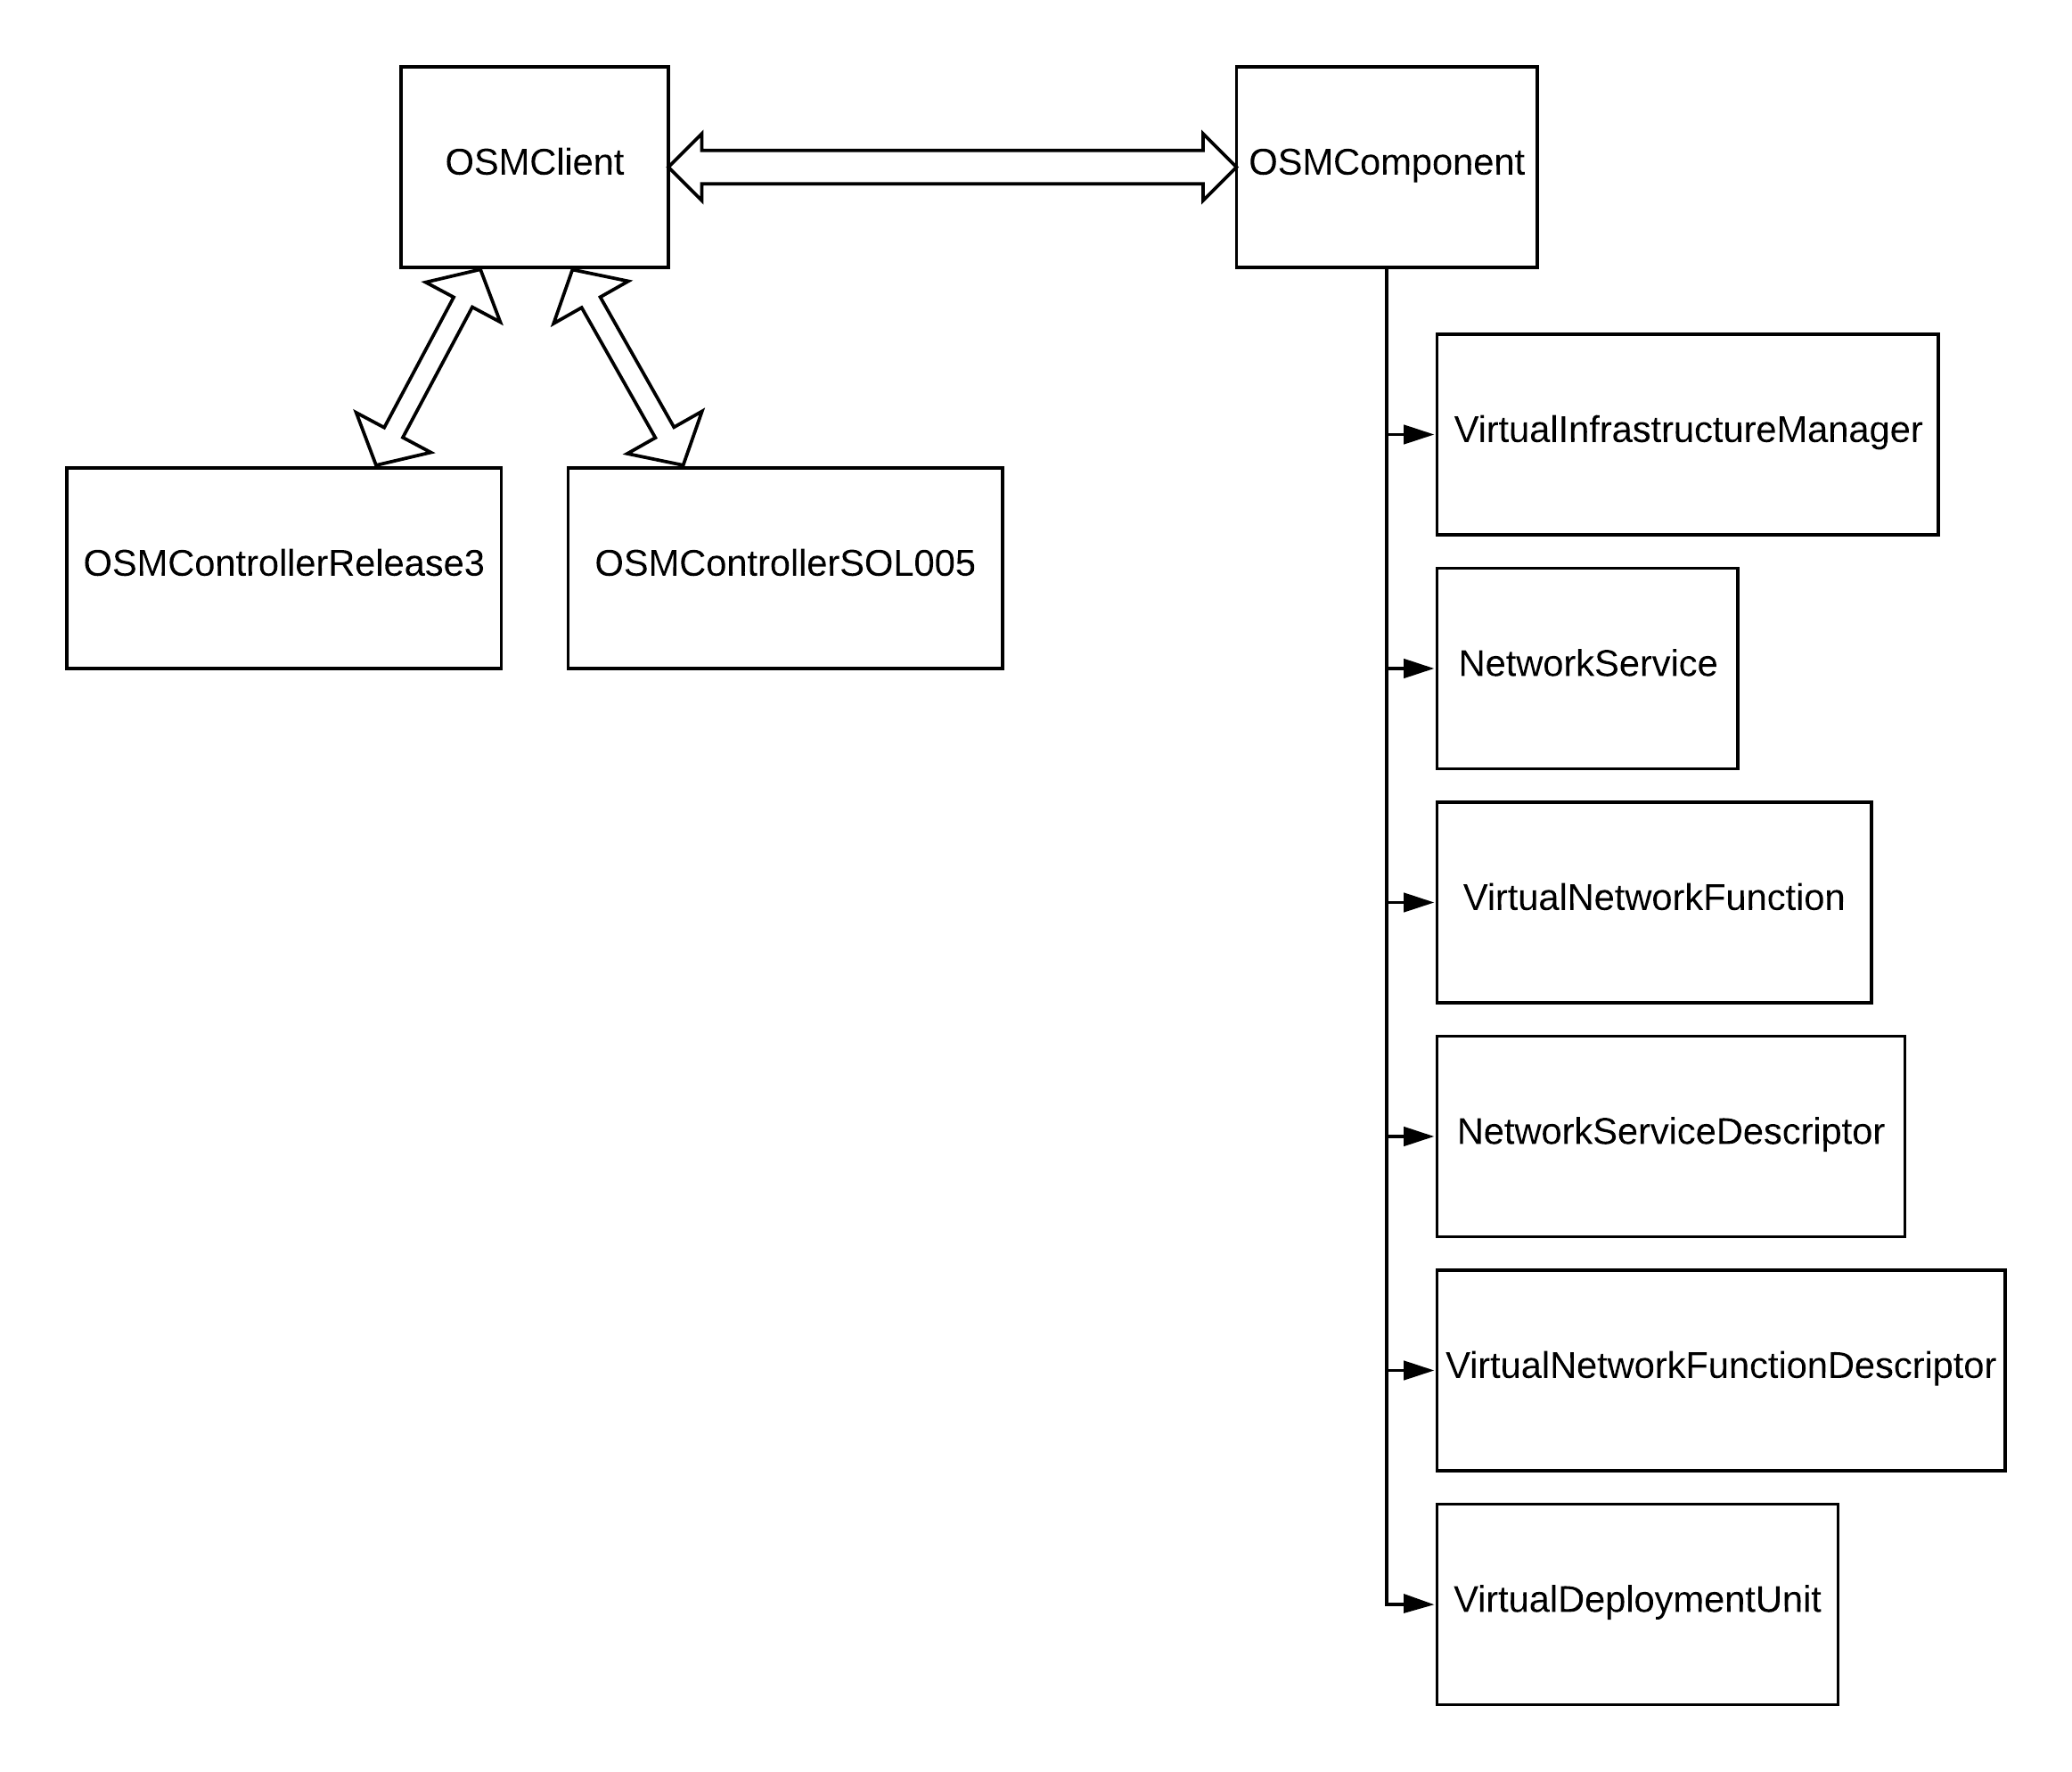
\includegraphics[width=1\linewidth]{imagenes/OSMClient}
	\caption{Estructura de clases de J-OSMClient}
	\label{fig:osmclient}
\end{figure}

En la figura \ref{fig:osmclient} se puede ver un esquema detallado de la jerarquía de clases. Se aprecia como OSMClient interactúa directamente con ambos \textit{controllers} para establecer la comunicación con ambas versiones de \ac{OSM}.

Así mismo, se pueden observar las clases auxiliares que definen los diferentes componentes internos de \ac{OSM}. Estas clases existen debido a que \ac{OSM} envía las respuestas \ac{HTTP} con un formato \ac{JSON}, que no es el formato óptimo para que el usuario final las reciba y las trate.

Estas clases auxiliares se explican a continuación:

\begin{itemize}
	\item \textbf{OSMComponent:} Es la clase genérica que define un componente de \ac{OSM}. Todas las demás clases heredan de ella, lo que permite un mejor procesamiento interno de las respuestas recibidas de \ac{OSM}, ya que proveé atributos comunes a todos los componentes, como nombre o identificador interno.
	
	\item \textbf{VirtualInfraestructureManager:} Esta clase es la que modela el componente \ac{VIM}. Proveé atributos como su \ac{URL} y su tipo (OpenStack, OpenVim, VMWare o \ac{AWS}).
	
	\item \textbf{VirtualLinkDescriptor:} Esta clase es la que define el componente \ac{VLD}. Proporciona un único atributo, que es una lista de conexiones en las que se indica los dos puertos que se conectan gracias a él.
	
	\item \textbf{VirtualDeploymentUnit:} Esta clase define el componente \ac{VDU}. Proveé diferentes atributos como la imagen que lo define y los recursos necesarios para su creación (Almacenamiento HD, número de CPUs y Memoria RAM).
	
	\item \textbf{VirtualNetworkFunctionDescriptor:} Esta clase es la que modela el componente \ac{VNFD}. Proporciona únicamente un atributo, que es la lista de \acp{VDU} que lo componen.
		
	\item \textbf{VirtualNetworkFunction:} Esta clase define el componente \ac{VNF}. Proveé diferentes atributos, como el \ac{NS} al que pertenece, el \ac{VIM} donde está instanciado o el \ac{VNFD} que lo define, entre otros.
	
	\item \textbf{NetworkServiceDescriptor:} Esta clase es la que modela el componente \ac{NSD}. Proporciona diferentes atributos, como la lista de \acp{VNFD} que lo componen o la lista de \acp{VLD}.
	
	\item \textbf{NetworkService:} Esta clase modela el componente \ac{NS}. Está compuesto de diferentes atributos, como los \acp{VIM} donde está instanciados sus \acp{VNF}, el \ac{NSD} que lo define, la lista de \acp{VNF} que lo forman o su estado actual.
	
\end{itemize}


\section{J-ONOS Client}
\label{sec:onosclient}

J-ONOSClient es una librería programada en Java cuya funcionalidad es la de proporcionar un cliente \ac{REST} para interactuar con \ac{ONOS} (ver \ref{sec:onos}). Esta librería está basada en la representación de objetos que proveé Swagger (ver \ref{subsec:openapi}). Gracias a Swagger, se puede generar automáticamente un cliente que interactúe con \ac{ONOS} en cualquier lenguaje de programación.

Este cliente generado proveé una representación de diferentes componentes, cada uno de ellos con una clase asociada que actúa como interfaz con \ac{ONOS} para controlar las interacciones que involucran a dicho componente. A continuación se explica cada uno de los componentes de \ac{ONOS}:

\begin{itemize}
	
	\item \textbf{Host:} 
	
	\item \textbf{Device:}
	
	\item \textbf{Link:}
	
	\item \textbf{Port:}
	
	\item \textbf{Flow:}
	
	\item \textbf{Intent:}
	
\end{itemize}


\begin{figure}[!ht]
	\centering
	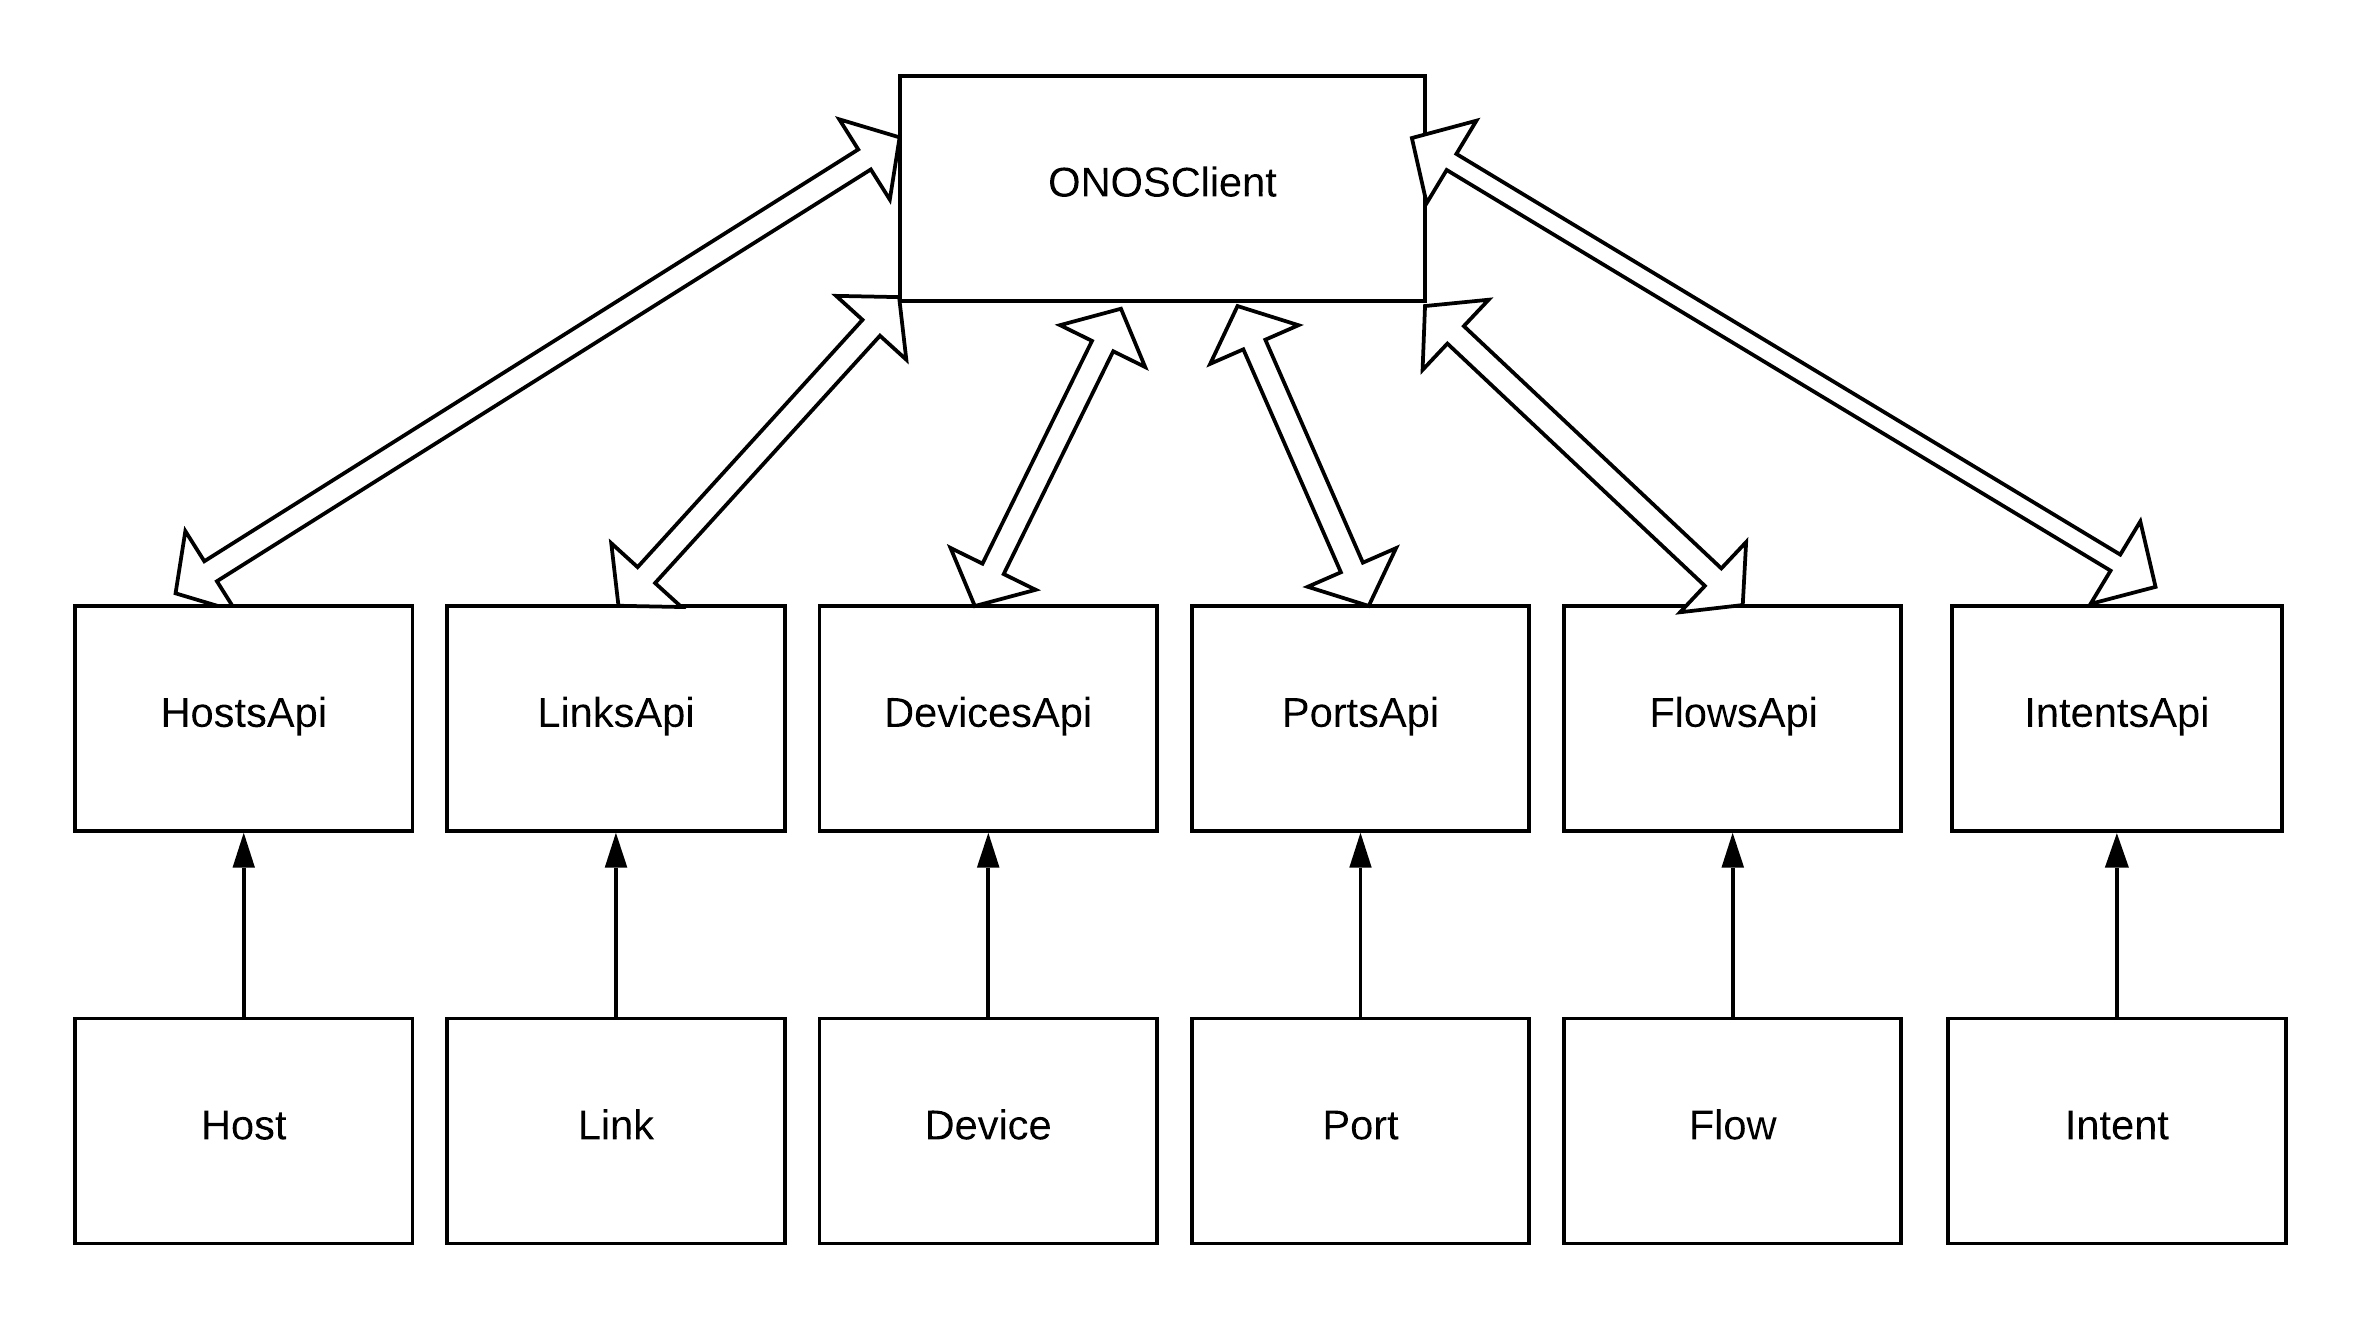
\includegraphics[width=1\linewidth]{imagenes/ONOSClient}
	\caption{Estructura de clases de ONOSClient}
	\label{fig:onosclient}
\end{figure}

En la figura \ref{fig:onosclient} se puede apreciar un esquema de la jerarquía de clases. 


\section{J-OpenStack Client}
\label{sec:openstackclient}

\begin{figure}[!ht]
	\centering
	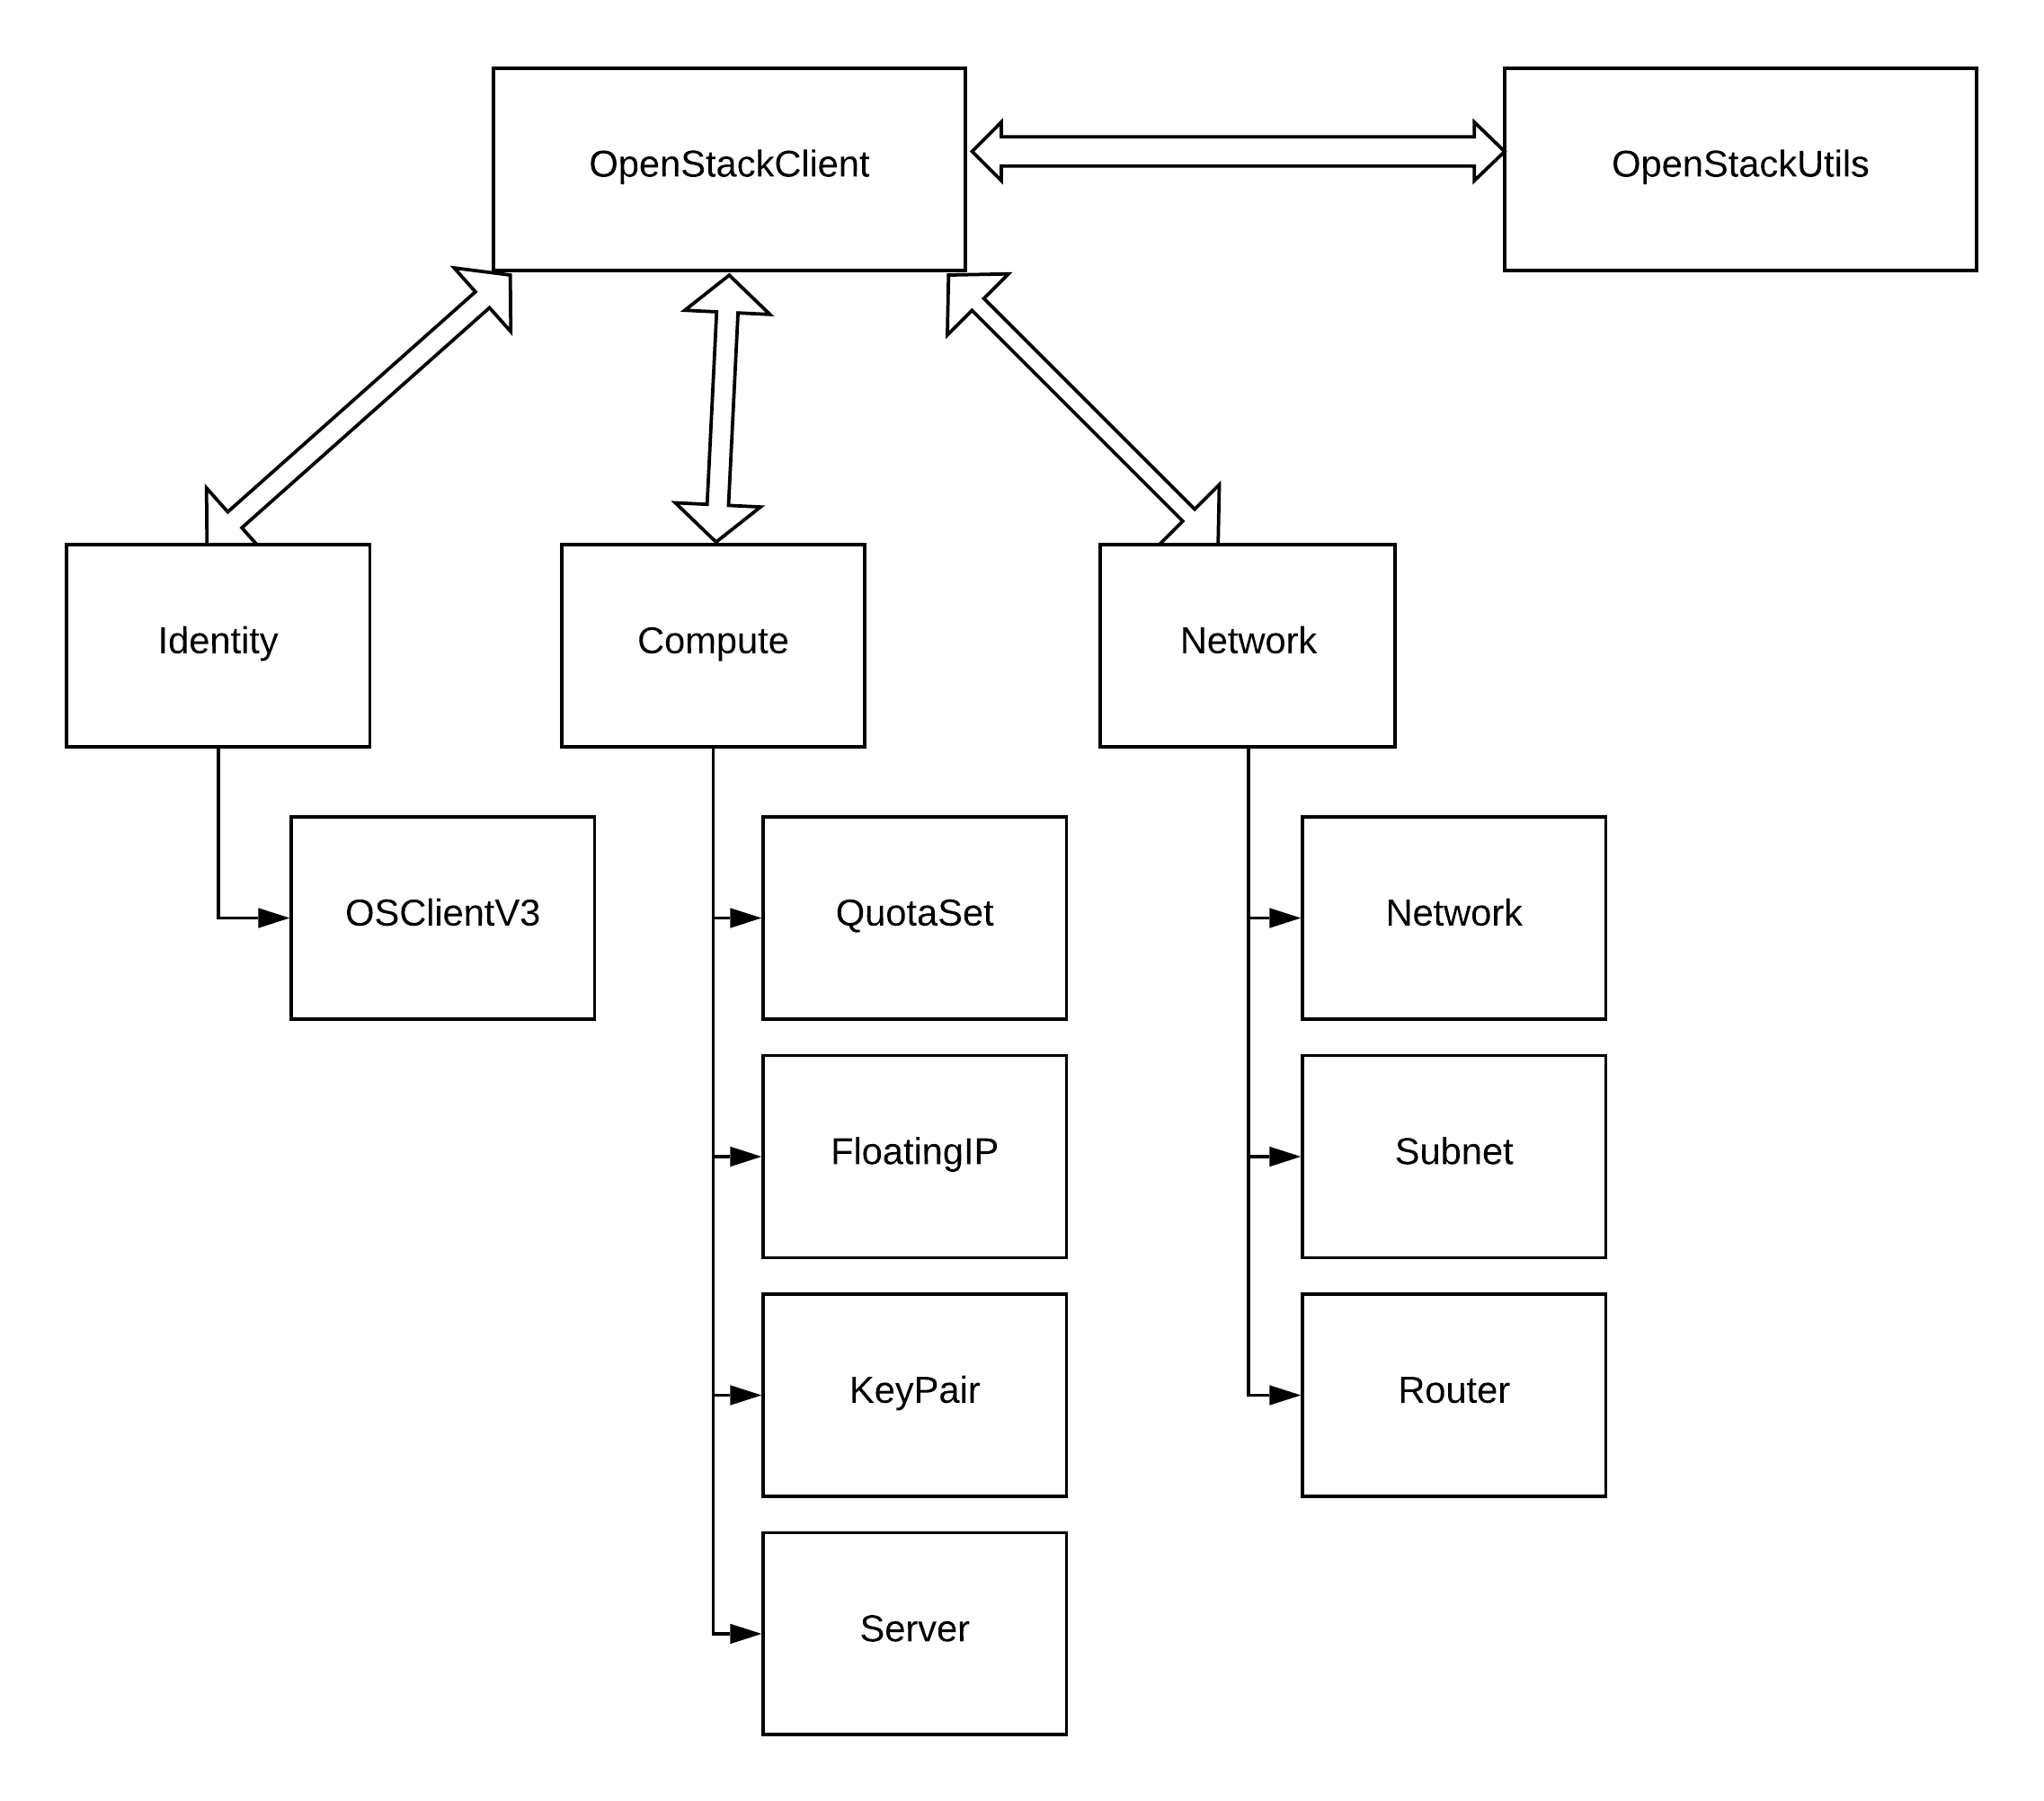
\includegraphics[width=1\linewidth]{imagenes/OpenStackClient}
	\caption{Estructura de clases de OpenStackClient}
	\label{fig:openstackclient}
\end{figure}

\section{Net2Plan: NFV Management Plugin}
\label{sec:nfvplugin}

Para llevar a cabo este proyecto, era necesario integrar las APIs mencionadas anteriormente con una herramienta que tenga funcionalidad de planificación de redes. Por ello, se ha desarrollado una extensión de Net2Plan basada en el plugin Network Design.


\begin{figure}[!ht]
	\centering
	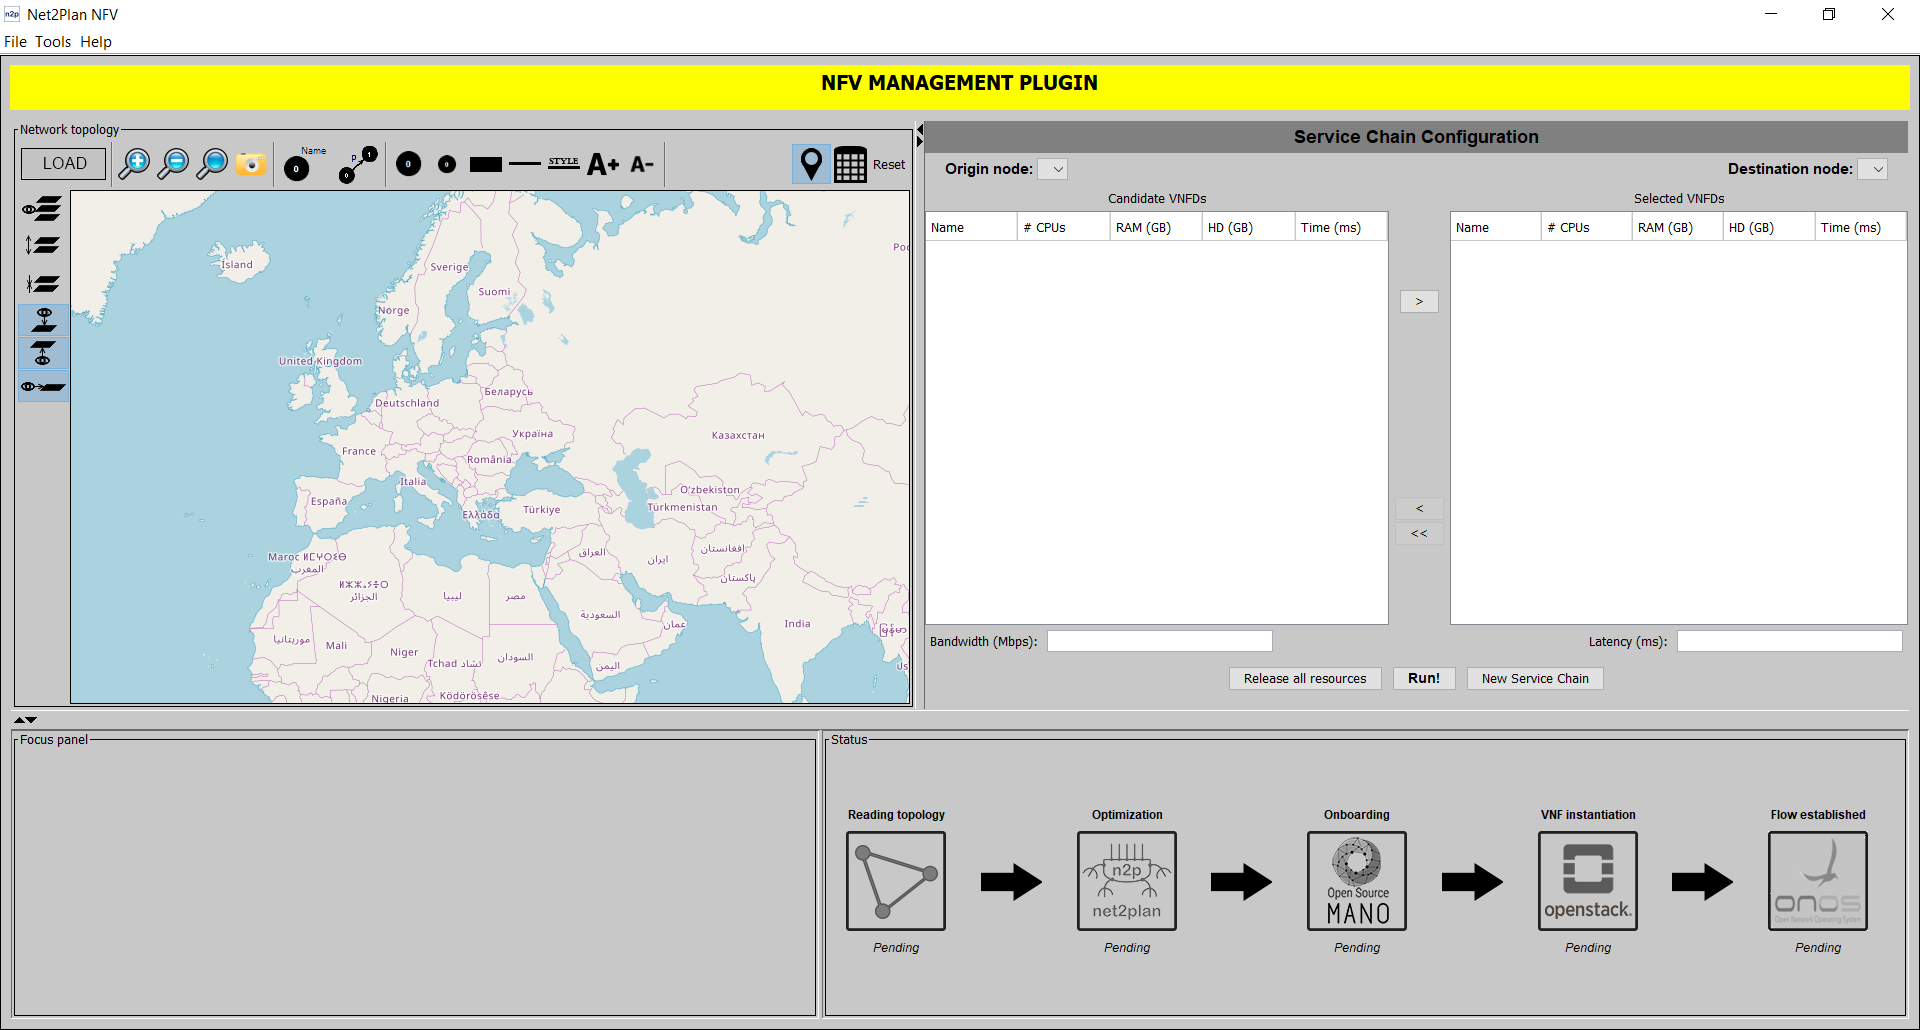
\includegraphics[width=1\linewidth]{imagenes/nfvplugin_dashboard}
	\caption{Interfaz gráfica del Plugin NFV-Management}
	\label{fig:nfvplugindash}
\end{figure}

Así mismo, en la figura \ref{fig:nfvplugindash} se puede observar la interfaz gráfica del Plugin NFV-Management, la cual está dividida en diferentes secciones:

\begin{itemize}
	\item Arriba a la izquierda se encuentra el \textit{TopologyPanel}, que se encarga de dibujar la topología deseada. Esta funcionalidad es heredada del \textit{Plugin Network Design} de Net2Plan.
	
	\item Arriba a la derecha se encuentra el \textit{OSMPanel}, que se encarga de obtener información sobre los distintos NSD que se encuentran disponibles en OSM y mostrarla al usuario de una manera amigable, informándole de que recursos (HD, RAM, CPU) son necesarios para su instanciación en un VIM.
	
	\item Abajo a la izquierda se encuentra el \textit{FocusPanel}, que se encarga de mostrar información detallada de un elemento en concreto cuando se selecciona. Dicha funcionalidad es heredada del \textit{Plugin Network Design} de Net2Plan.
	
	\item Abajo a la derecha se encuentra el \textit{ServiceChainPanel}.
\end{itemize}




\cleardoublepage